\documentclass[uplatex]{suribt}
%\documentclass[oneside]{suribt}% 本文が * ページ以下のときに (掲示に注意)
\usepackage[utf8]{inputenc}
\usepackage[japanese]{babel}
\title{超音波計測による深層学習を用いた菅内流体の相体積率推定}
%\titlewidth{}% タイトル幅 (指定するときは単位つきで)
%\centering
\author{松原貞徳}
\studentid{37246227}
%\eauthor{Sadanori Matsubara}% Copyright 表示で使われる

\supervisor{高木周教授}% 1 つ引数をとる (役職まで含めて書く)
%\supervisor{指導教員名 役職 \and 指導教員名 役職}% 複数教員の場合,\and でつなげる
\handin{2026}{1}% 提出月. 2 つ (年, 月) 引数をとる
%\keywords{キーワード1, キーワード2} % 概要の下に表示される
\usepackage{float}
\usepackage{amsmath} 
\usepackage[dvipdfmx] {graphicx}
\usepackage{amsfonts}
\usepackage{amssymb}
\usepackage{comment}
\usepackage{geometry}
\usepackage{bm}
% \usepackage{bbm}
\usepackage{subcaption}
\usepackage{url}
\newtheorem{lemma}{補題}[section]
\makeatletter
  % subsectionの下マージンを小さく
  \renewcommand{\subsection}{%
    \@startsection{subsection}{1}{\z@}%
    {0.4\Cvs}{0.1\Cvs}%
    {\normalfont\normalsize\headfont\raggedright}}
\makeatother
\begin{document}
%\Studentid{37246227}
\setcounter{tocdepth}{2}%\subsectionが目次に含まれるようにしている
% \begin{center}
% \Large{超音波計測による深層学習を用いた菅内流体の気相体積率推定}\\
% \normalsize{松原貞徳 指導教員 高木周教授}\\
% \normalsize{void fraction prediction from ultrasonic measurement technique using deep learning}
% \end{center}
\maketitle
\tableofcontents
\chapter{序論}
\section{研究背景}
数々の調査により、海底には豊富な海底資源が存在することが知られている。日本近海の海底資源を掘削、開発する研究は長年続けられてきたが、経済的な理由で実用に足る運搬手法は開発されていなかった。しかし近年では、メンテナンスが容易かつ運搬の仕組みが簡素であるとの理由でエアリフトポンプという機構が注目を集めている。この手法は海底に管をたてかけて、管内下部に資源と海水の混合流を流し込み、それらに圧縮空気を注入し空気が混合流と共に上昇しようとする力を利用して運搬を行うというものである。
当該手法の技術的課題としては、注入する空気の量を極めて厳密に制御する必要があるというものが挙げられる。空気が少なすぎれば運搬を行う能力が不足する一方で、注入量が多すぎれば流動の様式は環状流に推移し、大きく運搬性能が低下するという性質がある。効率的な運搬のためにはこれらの注入量を適切に制御する必要があり、管内の気相体積率を測定し制御の情報として利用しようとする案がある。しかし、そのような技術は現在開発されていない。運搬する流体は不透明流体であるとの理由から、従来支配的であった光やγ線を利用する方法は使用できない。また、鉱石を運搬する都合上、管にプローブを挿入するような侵襲的な計測手法は好まれない。\par
そこで注目されているのが超音波計測である。超音波はその反射波を測定し情報を利用することで不透明流体に対しても測定が行えると期待されており、また、流れに対して与える影響も無視できるほどに微弱である。海洋技術研究所で行われた実験データの提供を受け、計測された信号波形データと相体積率の間の関係性を解明し新たな計測技術の開発を行うことが期待されており、本研究室ではその協力を受けて技術開発を行った。
\section{関連研究}
エアリフトポンプを用い海底資源を揚降するプロジェクトが進行中であり、本研究室では開発の前段階としての性能評価の正当性を検証するため超音波計測による物理量の測定技術の開発が期待されている。より詳しく言えば、実海域において最適な管径や空気吹き込み条件を取得できればシステム設計にとって非常に望ましく、そのための構成方程式の精度検証により実測値を必要としている。

\subsection{エアリフトポンプを用いた揚降実験に関する研究}
\subsection{混相流の力学に関する研究}
\subsection{混相流計測手法に関する研究}

エアリフト揚降システムを開発する上で、入念な技術調査が行われてきた。流体力学においてはその計測手法が長らく研究されてきており、理論的工学的研究が数多く存在する。その中で、下にあるようないくつかの技術が検討された背景がある。\par
・写真計測\par
・締め切り法\par
・PIV,PTV\par
・電気プローブ、光ファイバプローブ、ワイヤメッシュなど\par
・X線・γ線\par
・静電容量方式\par
これらのうち、実験により写真計測、PIVなどの手法がまず検討されてきた。しかし、撮影された画像から有益な情報を得ることは困難であった。\par
次に、電気プローブ、光ファイバープローブ、ワイヤメッシュなどの方法が検討されてきた。しかし、これらは粗大固体粒子を含む系には適用不可という側面がある。\par
X線・γ線を利用する方法に関しては、固気液三相(三成分)だと体積率を取得する技術が存在しないことに加え、放射線を取り扱うので大口径化などの点で見通しが不透明であるという問題点があり、静電容量方式でも固気液三相だと体積率を得られず、軸対称性が崩れた場合などは計測できないことが予想されるのである。これらの理由により、超音波によって流体を計測する試みが行われてきた。様々な取り組みが各所で進行中であるが、例えば共同研究を行っている北海道大学においては純粋な物理学的アプローチに基づく技術開発が行われてきた。しかし、混相流には膨大な変数が存在しモデル化が極めて困難である。従来支配的であった光学的な計測も使用できず、また、光学的計測と異なり超音波計測においてはノイズの影響が極めて大きいことが実験的に知られており、信号波形から人為的に特徴を抽出するアプローチが限界に達しつつある。\par
本研究室においても諸先輩方によって研究がなされてきている。そのうち近年のものを簡単に紹介する。\par
例えば2023年には、管の断面を模した系での数値計算および、得られた信号波形をもとに気泡のサイズと位置を機械学習によって推定する研究がWangによって行われた。この中で、気泡がたった5つかつシミュレーションという条件下でも予測が困難であると指摘されている。しかし、データセットの統計に関する議論が行われていない。よりバランスされたデータを用いることによって再現できる可能性がある。また、その中で実機実験の必要性と3次元シミュレーション、固気液三相流のシミュレーションを行うことを提案している。\par
2024年には尾花によって上昇気液二層流の超音波計測の技術がまとめられ、超音波のTime-stripイメージをもとに学習させるアプローチにおいてスラグ流・チャーン流の識別が行われた。また、この中で数値計算による計測データを学習させることが提案されている。\par
2025年には渡辺によってCNNを用いた相体積率及び見かけ流速の推定が行われ、有効な前処理手法についての調査が行われた。その中で二相流においては高精度での推定が可能だが、固気液三相流では困難であると主張した。しかし、全体的にデータが極めて少なく、それゆえ十分なテストデータを用意できず、有効かどうかの検証が十分ではない。また、学習されたパターンの物理現象を、計算機理論と照らし合わせて議論する必要がある。

\section{研究目的}
以上に述べたとおり、従来の流体計測技術では当面の技術的課題を解決できず、我が国においては主に北海道大学と我々のチームで超音波での技術的開発が目指されてきた背景があり、本研究室においても技術的困難さが確認されている。前述のとおり系が極めて複雑であり、物理的な現象論的アプローチも限界に達しつつある。そこで、本研究においては複雑系の取り扱いに強みを持ち、それらの特徴、表現をデータから取得できる可能性のある深層学習の技術を用い技術的課題の解決を目的とした。とくに、相体積率を推定する目的のもと実験データおよび数値計算を活用してデータを入手し、現象論に基づいた考察を行うこととする。

\subsection{本論文の構成}
まず初めに研究の発端となった状況及びその動機に触れることによって動機を示し、そのうえで各所で様々な研究が行われてきたことを述べた。その中で顕著なものに焦点を当て、流体工学分野での混相流分野の概要や、流体計測技術を調査した。それを受けて、本稿において数値計算を活用して得られた知見やデータを信号処理によって適切に機械学習・深層学習と組み合わせ、目的の達成を図った記録を示す。その際、使用した技術を各分野ごとに分けて可能な限り綿密に記した。本稿の核をなす数値計算、そのデータの処理を体系づける信号処理、そして得られたデータをもとに予測を行う深層学習について概論を示し、それらに基づいて本稿における数値計算の結果とそれに基づく知見、さらにそのデータを学習させた場合の性能と評価、今後の展望を示す。
\chapter{技術的背景}
\section{超音波計測}
超音波とは振動である。それゆえ、媒体を必要とする。その媒体の物性によって減衰や反射の特性が変化するが、伝播した超音波、すなわち計測物体の振動の情報を圧電効果を利用することによって電気信号の形として取得し、適切に変換することによってはじめて信号波形を計測することが可能となる。それらは電子回路によって適切に処理され、信号波形として対象物を計測した際の情報を利用できる。本研究においては電気回路については簡単に触れるのにとどめることとし、あくまで取得された計測波形に基づいて議論を行う。

超音波を含む音は、周波数、強度、波形で表すことが可能である。すなわち$A$を振幅、$\omega$を各振動数、$\phi_0$を位相とした際に、音は 
\begin{equation}
    f(t)=Asin(\omega t +\phi_0)
\end{equation}
として表現されるので、周波数$f=\omega /2\pi$, 強度$I=\frac{1}{2}Z_0 A^2 \omega^2$, 波形$s$
として表現できる。  

超音波の性質として、周波数が高いほどまっすぐ進みやすい一方で、強度が減衰しやすいというものがある。超音波は物質の界面で反射する性質がある。これらの反射と入射・および減衰と透過の影響を特徴づける量が音響インピーダンス$Z = \rho c$(密度×音速)である。

$Z_0$が大きく異なる物質の界面では超音波は反射する。ゆえに超音波は液相から固相に入ることはできるが、気相に衝突した際にはほぼ全反射される。これらは実験的にも観察されている。
ゆえに、気液界面での超音波の反射を計測することによって鉛直管内流の気液界面を取得できる。

\section{音響信号処理}
これら超音波計測の際の信号を処理する方法論について述べる。これらについては音声信号処理に参考とすべき内容が多く、本研究に対しても有効と思われる手法に絞り紹介する。


\subsection{数理変換}
信号は目的に応じて適切に変換される必要があり、それを行う手続きは十分議論されている。フーリエ変換やヒルベルト変換は頻繁に用いられる。フーリエ変換においては定常性の仮定を置く目的でSTFTといった派生形があるが、今回は使用していない。ヒルベルト変換に関しては、変換に多大な時間を要するためにGPUでの計算を行う目的で

\subsection{超音波画像法}\label{ultraimage}
超音波画像は、特に医療分野で広く用いられている。妊婦のお腹の中の胎児を可視化しようとした場合には、人体に影響を及ぼす電磁波などよりも、力学的な刺激であり人体に無害な超音波を用いて可視化することが好まれる。ここで用いられているのが、超音波画像法と呼ばれる方法である。これは、超音波パルスを照射してその透過波、反射波を記録し、その強度に応じて色分けして表示することによって画像を得る手法である。これらは、一般に信号波形の包絡線を取得し、適切に対数圧縮を施すことによって実現される。

\subsection{ノイズ除去}
本研究における学習データに関してだが、計測機器の不具合といった何らかのエラーにより不適切な値を取ることがある。そういった値は適切な学習を阻害しうるので適切に除去する必要がある。これらに関してはデータ分布を適切な手法で確率分布としてモデル化し、値を取る確率が極めて小さいものを外れ値として除外するという案が考えられる。

\section{数値計算手法}
本研究においては、実機計測データに加え、シミュレーションによって生成した計測データも利用した。実機を模した機械学習用データを作成することを目的とした。

\subsection{計算原理}
超音波の伝播については波動方程式によってモデル化されており、系の時間発展を記述することが可能である。この方程式は原理的には二階の非線形偏微分方程式であるが、流体の保存則を活用することによって複数の一階偏微分方程式に分解することができ、数値的にも安定した計算が可能になる。

例えば、減衰なしの流体のもっとも単純な系の運動を記述する方程式として運動量保存則、質量保存則、圧力ー密度の関係式が存在する。これらはそれぞれ
\begin{align}
    \frac{\partial \mathbf{u}}{\partial t }&= -\frac{1}{\rho_0} \nabla p \\
    \frac{\partial \rho}{\partial t} &= - \rho_0 \nabla \cdot \mathbf{u} \\
    p&= c_0 ^2 \rho
\end{align}
が挙げられるが、これらを整理すると
\begin{equation}
    \nabla^2p - \frac{1}{c_0^2} \frac{\partial ^2 p}{\partial t^2} =0 
\end{equation}
の、波動方程式を得る。

すなわち、これらの波動方程式の解は、流体の保存則の解と等価である。
実際は減衰などのより現実に即した効果を付した項が追加され、より複雑な方程式となる。これらの式を離散化することによって、連続な量を対象とする本来の偏微分方程式を計算機で数値的に解くことが可能となる。

\subsection{疑似スペクトル法(pseudospectral method)}
シミュレーションにおいてはいくつかの数値的なモデルが存在する。そして、それらへの最適なアプローチは系に依存する。それらに対して、heterogeneous(不均質)な系、つまり様々な材質から成る系についての解を求めたいとする。こういった問題を解くには、有限差分法(finite difference)あるいは有限要素法(finite element)が考えられるが、有用な精度を達成するには音波長あたり10点が必要である。これらの方法では、過度に計算コストがかかってしまいがちである。

これらは、有限差分法が、もとの関数の近傍で近似を行うことに起因する。勾配を評価する際、高精度の値を得るにはより高次の多項式をできるだけ多くの点でフィッティングする必要がある。これらに対処するのがフーリエ選点法である。この手法は、データ点すべてにフーリエ級数を割り当てる。基底関数が正弦波的な形状を持つために、有限差分法と異なり高次の多項式を必要とせず、かつ2点でフィッティングできるので必要なグリッド数も少ないのである。よって、波動伝播においてはより効率的な計算手法であるとされる。

\subsection{安定性解析}
系の方程式を記述して、それを数値的に解く場合にはいくつかの検定が存在する。
\begin{description}
    \item[1.]離散化に伴う連続量との乖離
    \item[2.]安定性解析
    \item[3.]計算結果の正しさ
\end{description}

離散化に伴う量は、$\Delta t $を十分小さくとることによって導関数に一致することはここでは自明とする。よって、重要なのは数値的な誤差が時間発展によって増大してしまうか否かである。これらは、十分$\Delta t $を小さくとることが望ましい一方で、計算時間の制約からできる限り粗くとることが望ましい。しかし、ここでもいくつかの検定が存在する。ただし、一般に適切な領域で$\Delta t $を小さくとって計算をやり直し、その値が収束することによって正しさを証明する手法である。低周波の波長の伝播の計算はより高周波の伝播によって保障されているので、高周波の計算がそれを担保するのである。

\section{機械学習}
機械学習は、データからパターンを抽出する技術である。より詳しく言えば、入力と出力の関係をモデル化し、モデルによる予測結果と目標値との誤差が小さくなるようにモデルのパラメータを更新する技術である。このような更新を行うためには誤差関数の値を最も小さくする方向に適切にパラメータの更新量を求める必要があり、そのために誤差関数そのもののパラメータに関する勾配を評価する必要がある。パラメータの更新量を求める最適化アルゴリズムには、確率的勾配降下法(Stochastic Gradient Decent,SGD)に基づいた数々の手法が存在する。\par
この技術を駆使し、本研究では、超音波信号波形から相体積率を推定する回帰問題として定式化する。入力$\mathbf{x} \in \mathbb{R}^{1 \times W \times C}$($W$: 信号長、$C$: チャネル数)から連続値$y \in \mathbb{R}$(相体積率)を予測する関数$f: \mathbb{R}^{1 \times W \times C} \to \mathbb{R}$を学習する。

本研究では深層学習(CNN、Transformer)を中心としたニューラルネットワークアプローチを採用する。これらの手法は、信号波形から物理量を推定する関数を直接学習できる利点がある。


\subsection{正規化・正則化}
今回設計したモデルには、学習を円滑に行うためにいくつかの統計処理を施してある。今回、シミュレーションで得られるデータは数khPaにも及ぶ圧力変動であるのに対し実機試験で得られるデータはトランスデューサの―2~+2Vの範囲の電圧変化である。シミュレーションのデータを学習に利用し、実機データでの性能をテストするというアプローチをとるとは言え、そのままでは入力データにおける数値的な変動があまりに大きい。ゆえに、データのスケールをそろえるという操作が重要となる。このような操作は正規化と呼ばれ、単にシミュレーションと実機に見られる値の差異のみならず、同じ入力間のデータや、隠れ相を通った後のデータに対しても同様に重要である。

\subsection{モデルの種類と概要}
深層学習の技術はデータが大量に存在し、モデルが不明であり、かつ「存在するとわかっている」ような分野において発展してきたという背景がある。Transformerとは自然言語処理の分野で考案されたアルゴリズムであり、自然言語のみならず画像処理、系列処理といった様々な分野に応用され、従来のアプローチの性能を大きく上回るという研究成果が様々な分野において発表されている。

本研究では、特徴、表現をデータから取得できる可能性のある深層学習の技術を用い技術的課題の解決を目的とした。とくに、相体積率を推定する目的のもと実験データおよび数値計算を活用してデータを入手し、現象論に基づいた考察を行うこととする。
\subsection{モデル解釈}
CNNやほかのアーキテクチャで学習された特徴の解釈に用いられる方法はいくつかある。例えば、学習したカーネルそのものをプロットする方法である。これらに関しては、深層学習の際に用いたカーネルをすべてプロットするというものである。一般に、\cite{Bishop:DeepLearning24}にあるように、下層のカーネルほどエッジのような機械的な特徴を、上層に行くほど高次の概念を学習していると解釈される。\par
一方、入力のどの領域が予測に最も寄与しているかを可視化する方法として顕著性map(saliency map)というものがあげられる。これらは、入力のどの領域に大きな重みを割り当てているかを確認する方法である。その最たるものがGrad-cam\cite{Selvaraju_2019}と呼ばれる方法である。これらの機能の詳細に立ち入る前に、その応用例に焦点を当てる。以下は、原論文にあったような、自然画像を入力として分類を行うモデルである。
\begin{figure}[htbp]
    \centering
    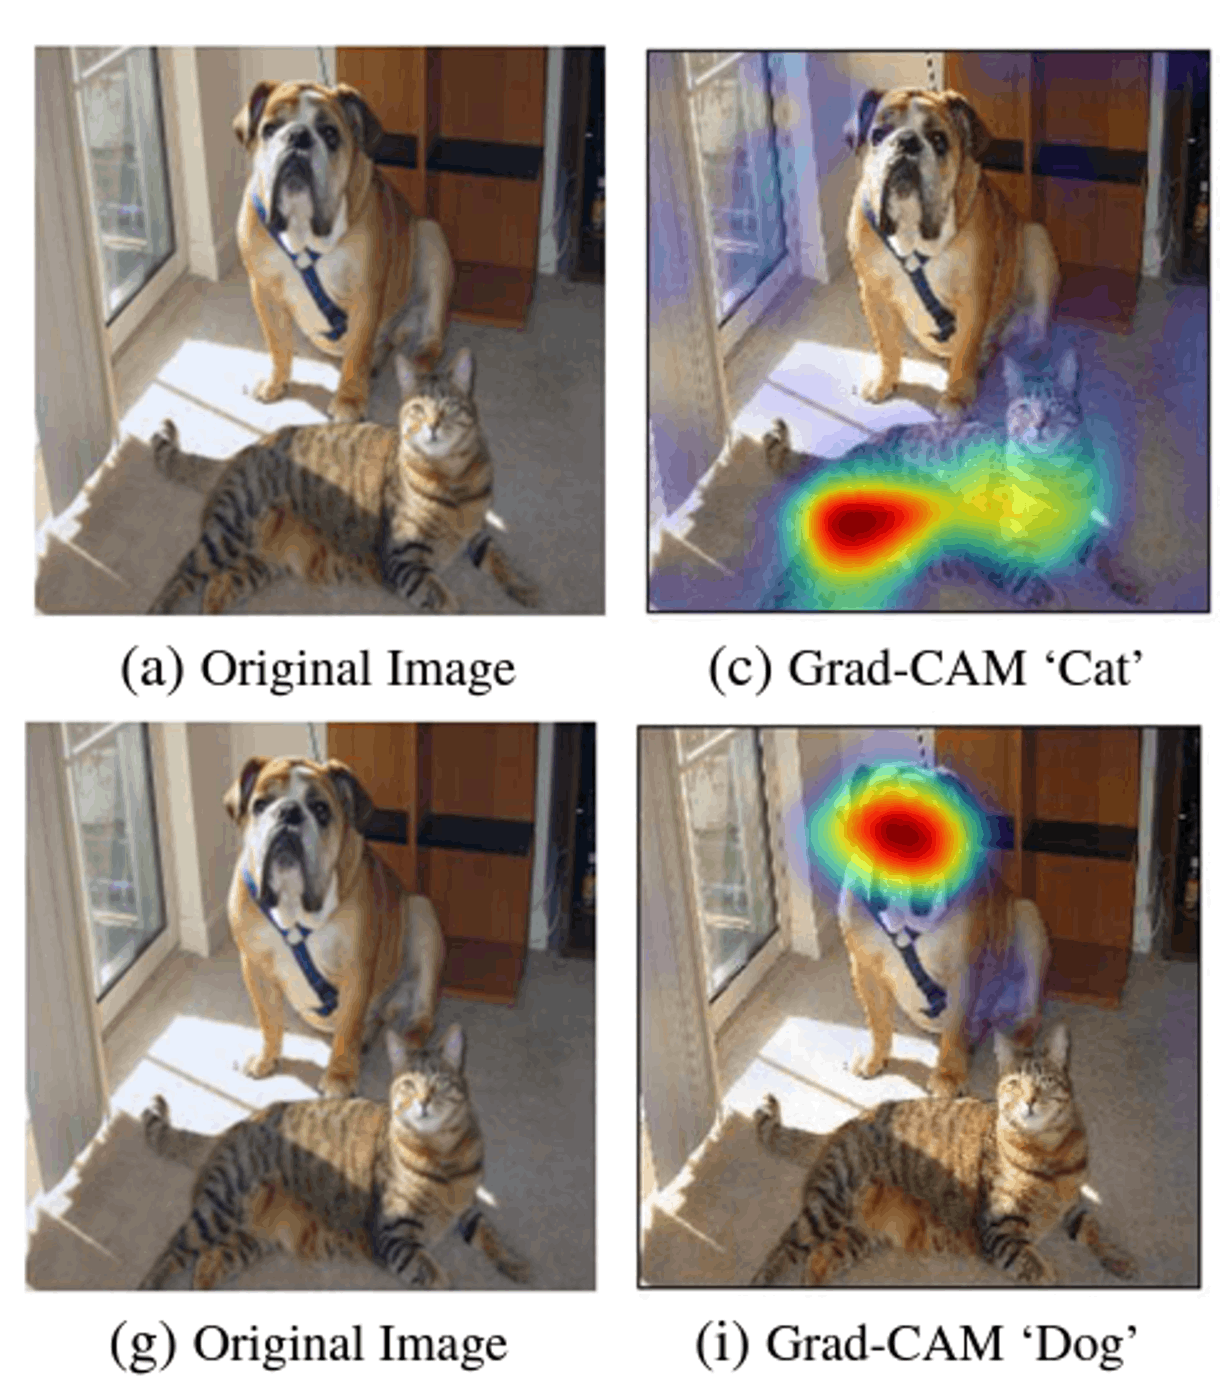
\includegraphics[width=0.5\linewidth]{pictures/explanation/grad_cam_explained.png}
    \caption{画像入力に対するsaliency mapを可視化したもの。1枚の画像に犬と猫が映っているが、犬、猫それぞれのクラス予測に対応する入力箇所が可視化されている。}
    \label{fig:gradcam}
\end{figure}
ある画像に犬が含まれるか、猫が含まれるかを識別する場合は、まずそのカテゴリに属する確率を計算し、そのうえで最大の確率を持つクラスに割り当てるという処理がされる。(Decision theory, 決定理論と呼ばれる)注意すべきは、この画像には、犬に属する確率も猫に属する確率も等しく存在する点である。その上で、Gradcamは、畳み込み層最終の出力の変化が、Softmax関数に通す前の値にどれだけの変化を起こすのかというものを可視化する。式で言えば、
\begin{equation}
    \alpha_k=\frac{1}{M_k}\sum_i\sum_j{\frac{\partial a^c}{\partial a_{ij}^k}}
\end{equation}
の値を計算し、これらの重みでもって最終層を強調する。
強調すべきは、ニューラルネットにおいては全く同型の写像の機能を持つ関数が学習された場合でも、別々の重みが得られるということである。Bishop\cite{PRML}によれば、これらは同様に良いモデルであるとされる。しかし、今回のような事例では、ある重みのセットよりも好まれる重みのセットが存在する。実機試験においては超音波パルスの形状が機器の性質により扁平になってしまうケースがあり、予測に寄与しない部分にまで同様の重みを割り当てるモデルはロバストな予測に寄与しない。これも結果の章で議論してある。
\chapter{実験手法・実験系}
\section{実験装置・計測機器}
協力を受けた海洋技術安全研究所の実験設備を以下に示す。
産業技術総合研究所の実験設備の写真を以下に示す。これに関しては、超音波計測が不十分であったため解析も検証も行っていないが、大まかなイメージを掴むために掲載することにする。
これら実験系は、上昇鉛直管における固液二層流、気液二層流、固気液三相流を超音波で計測した場合の信号データのほか、空間平均の相体積率や画像データに関しても取得できることが目的とされており、いくつかの設備が複合されてある。信号データを取得する目的でトランスデューサが、画像データを取得する目的で超音波照射と同期する設定のもとハイスピードカメラが設置されている。なお、空間平均の相体積率は締め切り法と呼ばれる手法で計測されており、これは上下バルブを同時に遮蔽し、バルブ間に取り残される媒体を測定する手法である。固相に関してはガラスビーズの個数が数えられ、気相、液相に関しては液相のみ体積率の比として測定される。1から液相、固相の割合を引くことによって気相の体積率が求められる。
概念図を以下に示す。この図のポンプにより流体の駆動力を得、適切に空気を注入することによって混相流が再現される。
\section{実験条件・手順}
これら実験系は、上昇鉛直管における固液二層流、気液二層流、固気液三相流を超音波で計測した場合の信号データのほか、空間平均の相体積率や画像データに関しても取得できることが目的とされており、いくつかの設備が複合されてある。信号データを取得する目的でトランスデューサが、画像データを取得する目的で超音波照射と同期する設定のもとハイスピードカメラが設置されている。なお、空間平均の相体積率は締め切り法と呼ばれる手法で計測されており、これは上下バルブを同時に遮蔽し、バルブ間に取り残される媒体を測定する手法である。固相に関してはガラスビーズの個数が数えられ、気相、液相に関しては液相のみ体積率の比として測定される。1から液相、固相の割合を引くことによって気相の体積率が求められる。

\section{データ取得方法}
本研究における学習データに関してだが、計測機器の不具合といった何らかのエラーにより不適切な値を取ることがある。そういった値は適切な学習を阻害しうるので適切に除去する必要がある。これらに関してはデータ分布を適切な手法で確率分布としてモデル化し、値を取る確率が極めて小さいものを外れ値として除外するという案が考えられる。

今回、実機データとその際の測定記録を拝見した際には、恐縮ながら命名が誤っていたり、データが破損している事例がしばしば見られた。例えば、実機測定データは存在するがそれらに対応する相体積率の目標値がなかったり、その逆がみられた。これらは筆者が手作業で確認し、修正した。今後このデータに基づいて解析を行う場合には、解析の担当者の負担が増すことがあるので、注意されたい。

また、後述するように、実機データにおいてはシミュレーションと異なり尖ったピークは一般に現れない。実際には尖った先端を切り取って台形にしたような信号波形になることが確認されている。これらに対し、適宜関数をフィッティングしてピークを補完し、より正しい値でのスケーリングを行うことが考えられる。その技術は、例えば\cite{kyodaisenpai}の技術を使えば解決できる可能性はある。
\chapter{計算系}
本研究においては、実機計測データに加え、シミュレーションによって生成した計測データも利用した。すなわち、シミュレーション生成のデータをもとに機械学習モデルを訓練・検証した後に実機データにおいてそれを評価するモデルも存在する。実機を模した機械学習用データを作成することを目的とした。

\section{計算系の設計}
数値計算を実行するためのオブジェクトを点群として定義し、それらに対し適切な物性値や信号遅延などを与えることによって実機に近い測定データを得ることが可能となる。計算系において存在する媒質は、固気液三相流の場合も含め石、塩化ビニル、水、空気、ガラスであり、これらをトランスデューサによって計測するという設定をなす。一般的な設定において、2次元では任意のセンサー配置ができる一方、現実の測定に即したビーム収束などは再現できない。一方、3次元では送信器、受信器でそれぞれ一つのトランスデューサしか実装できないが、各素子への信号の送信に時間遅れを持たせて、超音波に指向性を持たせることが可能となる。計算に使用した各種物理量はconfig.jsonにも記載されているので、そちらを参照されたい。以下は、それぞれの設定理由を示す。
\subsection{グリッドサイズ}
次に、計算を行う上では格子点、その幅を計算機の性能を鑑みながら決定しなければならない。理想的には、計算機の性能が、シミュレーションに必要な性能を大幅に上回っている状態が望ましく、計算機の制約を考えずに設計したい。しかし、研究室の計算環境ではやはりそれも考慮して計算系の設計をする必要があった。以下、計算系の要件を示す。\par
まず実験設備のスケールとしては、トランスデューサが超音波を照射しその反射波を記録する目的から、
\begin{equation}
    l_x\ [\mathrm{mm}] > 82 \ \mathrm{mm}
\end{equation}\par
である必要がある。また、幅に関しては管の直径よりも太くある必要があるので、
\begin{equation}
    l_y \ [\mathrm{mm}]> 32 \ [\mathrm{mm}]
\end{equation}
が必要である。
なおこれらは下限であり、実際はもう少しゆとりを持たせることが好まれる。\par
他方、計算を正確に行うための計算理論による要件を示す。先に述べたように、波動の位相を正確に取得するためには、$\lambda_{min}=c_{min}/f$,$c_{min}$を、系の構成要素の中での最も遅い伝播速度として
\begin{equation}
    2 \Delta x\ [\mathrm{m}] < \lambda _{min}\ [\mathrm{m}]
\end{equation}
である必要がある。
例えば固液二層の場合では律速が水なので$c_{min}=1500 \ [\mathrm{m/s}]$, 気液・固気液では空気が律速となるので$c_{min}=340 m/s$となる。
ゆえに、例えば固液を例にとると、現在使用している超音波の波長が$4 \ \mathrm{MHz}$であるので
\begin{equation}
    \Delta x \ [\mathrm{m}]< \frac{1500}{2 \cdot 4 \cdot 10^6} \ [\mathrm{m}]= 0.1875 \ [\mathrm{mm}]
\end{equation}
を満たさなくてはならない。ただし、2倍、3倍などの高周波成分などの量を再現しようとした場合には、その分だけ小さくとる必要がある。これらは、フーリエ変換のスペクトルで$12 \ [\mathrm{MHz}]$のピークがわずかに見られたためそれらを再現する目的で$0.0625 \ [\mathrm{mm}]$よりも小さい値に設定する必要があった。\par
ここで、格子点数の要件について記す。今$l_x =N_x \cdot dx > 82 \ \mathrm{mm}$であるので、
\begin{equation}
    N_x > 1312
\end{equation}
が示される。計算機上は2の累乗だと計算効率が良いので、$N_x=2048$を採用してある。
同様の議論で$N_y > 512$が必要だが、これでは計算系の境界に接してしまうので望ましくない。そこで、それよりも大きくかつ効率が良い値として$N_y=768$を採用した。\par
最後に、$N_z, dz$について触れる。これらは、計算機の上限から$N_z=128$とした。これらによりGPU上で20GBの仮想メモリが割り当てられ計算が実行された。
\subsection{固液二層流}
系を規定する媒体は、ガラスおよび水の二種類である。また、実験記録にはガラスビーズの直径が2.5 mmと記載されてある。よって、事前にガラスビーズの個数を規定しておき、それを空間的に配置して計算系を作成した。この際、複数のガラスビーズの座標はBox-Mullar法と呼ばれる乱数生成のアルゴリズムをベースに、適当な検定を設けることによって生成した。以下にその詳細を示す。これらによって生成した座標は$\{x | x\in[-1,1]\},\{y | y\in [-1,1]\},\{z |z \in [0,1]\}$ の区間で生成されており、これをグリッドサイズの分だけ拡大することによって計算系の座標として利用してある。
トランスデューサの設定としては以下のものを用いた。


\subsection{気液二層流}
今回は空気と水の二種類によって系が決定される。固液二層との違いは、気泡の形が球形を成すとは限らず、またその形状も複雑であり、体積も一定でないということである。著しく非軸対称であり、分裂の最中のもの、合体の最中のものなど混迷を極める。一方で、気液二相に関しては画像解析に基づくいくつかの知見が存在しているのも事実である。例えば坂口ら\cite{sakaguchibubble}の研究によれば、大きい気泡は菅中央に、小さい気泡が間壁付近に分布することが明らかになった。また、古典的な教科書である\cite{batchelor2000introduction}によれば、$6\times 10^{-4}c.c$程度の小さい気泡に関してはほぼ球であると仮定してよく、この値を超えると扁平となり振動しながら上昇する。次に、体積が5ccよりも大きくなると球の一部を切り取ったような形になり、また、その仰角は泡の体積によらず46°~64°となる。最後に、菅いっぱいを占めるような大きな泡に関しては、形状定数$\alpha$、気泡の上昇速度$U$,重力加速度$g$、よどみ点における気泡表面の曲率半径$R$を用いて
\begin{equation}
    \alpha^2 U^2 = gR
\end{equation}
の形状をなす。また、$U$は円管の内径を$D$として$0.48\sqrt{gD/2}$に等しく、$R/D>0.26$ならば半径$R$の帽子型形状の泡よりも小さい。ゆえに、管を埋めるほど大きくない泡は大きい泡へと追いついて合体することを示すという。最後に、これら帽子型から十分下方では、質量保存の式から
\begin{equation}
    \pi \frac{D^2}{4} U=\pi {\frac{D^2}{4} - (\frac{D}{2}-d)^2}\sqrt{2gx}
\end{equation}が得られ、基本の先端からの距離を$x$として
\begin{equation}
    \frac{2d}{D} =1 -\sqrt{1-\frac{U}{\sqrt{2gx}}}
\end{equation}
の関係式を成すという。さらに、村井の研究\cite{村井祐一20222022.T011}らにより気泡径とその分布が統計されており、その形状は、ポアソン分布に酷似している。
これらから、技術的に大まかにモデル化可能な領域と、その正しさが確認される。すなわち、超音波伝播をシミュレートする上で気泡の数$N$、形状の関数$S_i$、気泡それぞれの座標$\mathbf{r}_i$を決定する必要がある。ここで、形状のモデル化に関しては極めて難しいので、構成要素としては球あるいは円柱を組み合わせただけとする著しい簡略化を行った。ゆえに、これら形状は球の直径$D_i$と円柱の高さ$h_i$の関数としてよく、また、座標$\mathbf{r}_i$の確率分布は$D_i$によって規定されると仮定できる。
これらから、暫定的に条件を満たす分布を以下のように定義して以下議論を進めることとする。$N$は既知とする。

\begin{align}
    &D \sim Pr(\nu) \\
    &h \sim Uni[0,a] \\
    &S =\left\{ \,
    \begin{aligned}
        &Sphere  (0 < D < 1 mm) \\
        &Oblete (1< D <10 mm)\\
        &Spherical-cap (10mm< D )\\
        &fill-bubble 
    \end{aligned}
\right.
\end{align}\par
ここで、spherical -capに関しては仰角が46~64°と定まっているため、60°と定義することによって、曲率半径$R$の関数として体積を導出できる。高校レベルの数学でこれは計算可能で、$\theta=\pi/3$の時は
\begin{equation}
    V(R)=\frac{16-9\sqrt{3}}{24}\pi R^3\sim0.0539R^3
\end{equation}
と計算できる。これらを実装することにより、上昇気液二層流における気泡流、スラグ流、チャーン流、環状流のうち気泡流と環状流のシミュレーションを行えることが期待される。スラグ流・チャーン流は著しく不規則なので、大変な技術的困難が予想される。


\section{数値計算結果}
実際の数値計算による結果と、その概要を示す。目安として、研究室の計算環境であるNvidia RTX 4090を利用した場合には、1データあたりおよそ4時間を要した。前節での物性値をもとにして数値計算を行った。
\subsection{液相のみ}
まず、液相のみのシミュレーションが妥当かどうかを実機をもとに検証する。
\begin{figure}[htbp]
    \centering
    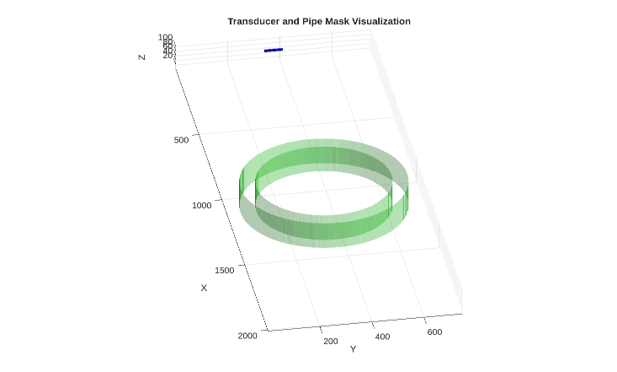
\includegraphics[width=0.5\linewidth]{pictures/results/liquid_only.png}
    \caption{数値計算の計算系の模式図。緑色のものがパイプを模しており、周りを水で満たしているものとする。}
    \label{fig:calculation_system}
\end{figure}出力された結果は以下のようなものであった。
\begin{figure}[htbp]
    \centering
    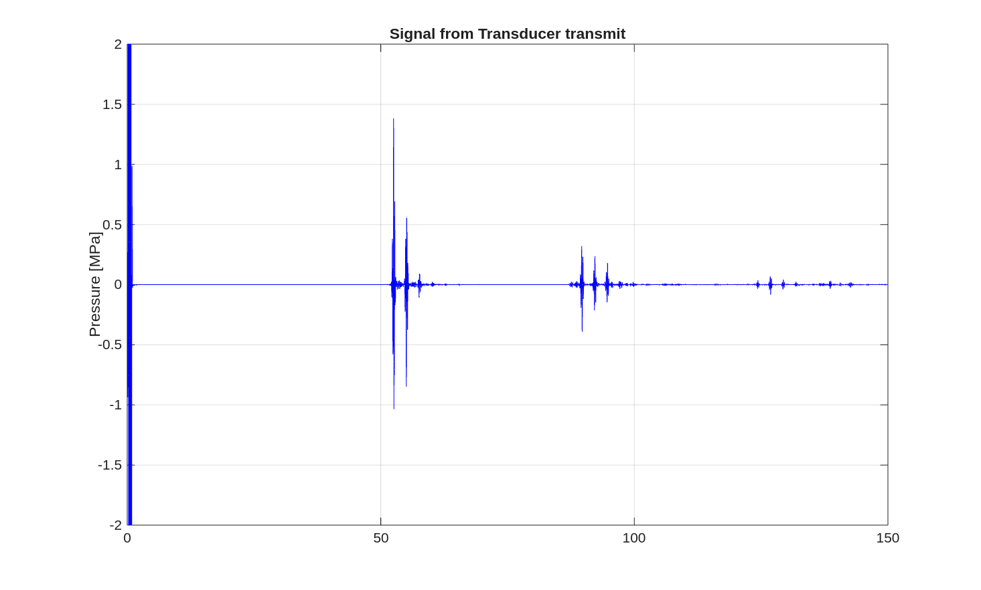
\includegraphics[width=0.5\linewidth]{pictures/results/liquid_only_signal.png}
    \caption{液相のみの場合の信号波形}
    \label{fig:liquid_only}
\end{figure}
液相のみの条件に関しては実際に実験されており、以下のような結果が存在する。一つのデータを示す。
これらの信号波形について、より詳細な解析を行った。
また、シミュレーション生成の信号のうち、管壁からのものを詳細に解析する。信号に対してはヒルベルト変換により検波処理を行っており、包絡線を取得してある。このとき、以下の結果が得られる。
\begin{figure}[htbp]
    \centering
    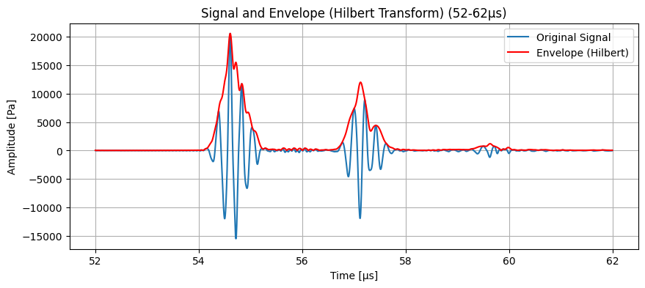
\includegraphics[width=0.5\linewidth]{pictures/results/pipe_refrection_sim.png}
    \caption{Caption}
    \label{fig:pipe_reflection}
\end{figure}
\begin{figure}[htbp]
    \centering
    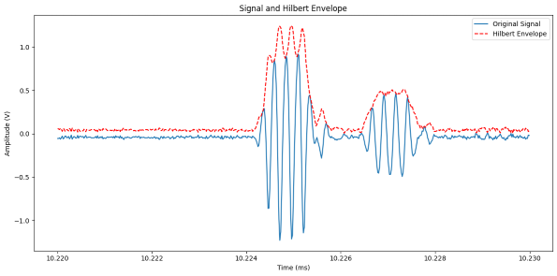
\includegraphics[width=0.5\linewidth]{pictures/results/pipe_refrection_real.png}
    \caption{Caption}
    \label{fig:pipe_reflection_real}
\end{figure}
これらを比較すると、定性的にはシミュレーション側では山のような形になっており、4回繰り返した信号波形のピークが見えにくい一方で、実機実験の方では先がつぶれたような形状をしていることがわかる。
これらのピークの間の時間差を取得することによって、材質がわかればその厚さが、厚さがわかれば媒体中の音速並びに材質が決定できる。
時刻0を、超音波を照射したタイミングとする。この際、\cite{塩ビ2021}を含む数々の資料でパイプの材質は塩化ビニルだと報告されており、\url{https://ims.evidentscientific.com/}によれば$2395\ \mathrm{m/s}$の伝播速度を持つ。一方で、実測データのピークを詳細に図ると往復で$2.15 \pm 0.019\ \mathrm{\mu s}$の時間差を持つ。これらから算出される厚さは$2.58\ \mathrm{mm}$となるが、事前に報告されていた値である3㎜と合わない。一方で、厚さを$3\ \mathrm{mm}$と仮定した場合の音速は$2790\ \mathrm{m/s}$となり、対応するパイプの材質は「アクリル」となる。\par
今回は情報が不足しているため、材質をアクリルだとみなし音速の値としては$2790\ \mathrm{m/s}$を採用した。
次に、この領域に対してフーリエ解析を実行した。まず、実機データのパイプ部分に対する周波数成分を解析する。
\begin{figure}[htbp]
    \centering
    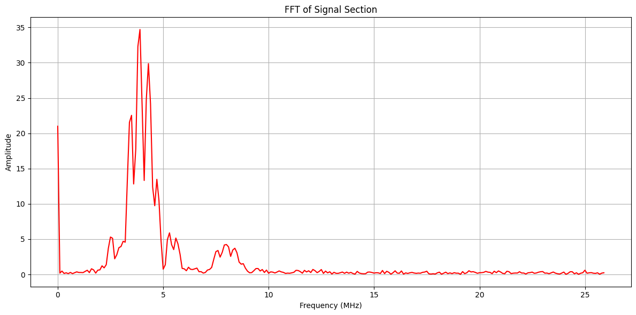
\includegraphics[width=0.5\linewidth]{pictures/explanation/Fourier_analysis_real.png}
    \caption{Caption}
    \label{fig:fourier_analysis_real}
\end{figure}
これらから、定性的には$4,8\ \mathrm{MHz}$の地点にピークがみられる。使用しているものとちょうど倍の周波数成分がみられるが、これらは倍音(second harmonic)と呼ばれる。\par
次に、数値計算によって生成した信号に対するフーリエ変換を行った結果を示す。以下は$CFL=0.03$で行ったものである。
\begin{figure}[htbp]
    \centering
    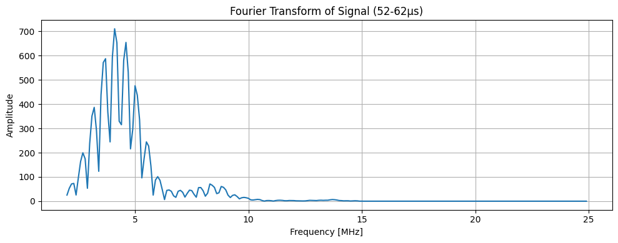
\includegraphics[width=0.5\linewidth]{pictures/explanation/fourier_analysis_sim_0.03.png}
    \caption{CFL=0.03に対する信号波形のフーリエ解析結果。実機と同じ4,8にピークがみられる。}
    \label{fig:fourier_analysis_sim_003}
\end{figure}
次に、$CFL=0.01$で行った結果を示す。
\begin{figure}[htbp]
    \centering
    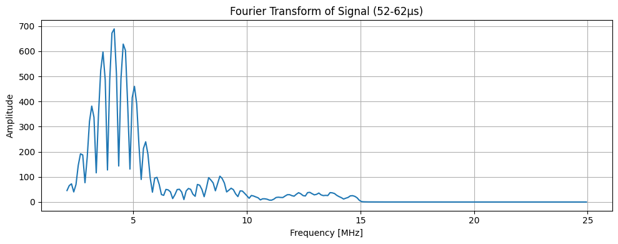
\includegraphics[width=0.5\linewidth]{pictures/explanation/Fourier_analysis_sim_0.01.png}
    \caption{CFL=0.01に対する信号波形のフーリエ解析結果。実機にはない12の成分を持っている。}
    \label{fig:fourier_analysis_sim_001}
\end{figure}
これらから、周波数空間の観点から、CFLの値としては0.03が好ましいとした。一方で、これらは計算の成立条件を満たしている(\ref{appendix})ので、以下すべてのシミュレーションはこの値のもと行った。
\subsection{固液二層}
3次元シミュレーションによって計測信号波形を生成した。これらは、機械学習用に使用するものである。基本的に機械学習用データは多いほうが望ましいが、多数は不可能であった。故に100ほどのデータを生成し、それによって訓練を行った。その結果を以下に示す。
\begin{figure}[htbp]
    \centering
    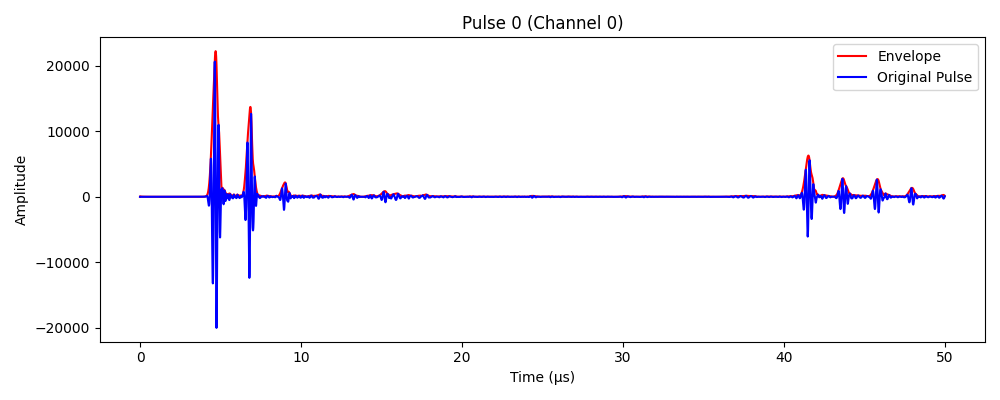
\includegraphics[width=0.5\linewidth]{pictures/results/solid_liquid7_processed_0pulse.png}
    \caption{固相粒子を含めた場合の信号波形}
    \label{fig:solid_liquid}
\end{figure}

\chapter{提案手法}
今、適当な何らかの測定を実行している間、その測定領域における真の値が存在する。これらによって超音波の信号波形が何らかの影響をうけて、測定結果として入手することができる。すなわち、今回の場合は相体積率が潜在変数、測定信号が確率変数として議論を進めるのが適切である。\par
ここで、信号波形から体積率を求めるのと逆の場合、すなわち体積率から信号波形を求める順問題は、比較的容易に解くことができる。固相粒子の個数および一つの粒子の体積、およびその相配置が既知とした場合には、波動方程式に基づく数値的な反復法によって超音波パルスの伝播を再現することができる。よって、数値計算シミュレーションソフトウェアを使用し、ある相体積率及びその相配置に基づく信号波形を生成した。\par
信号波形からそれに対応する相体積率を機械学習で推定する手法の一つには、連続値を推定する回帰モデル、すなわち
\begin{equation}
    p(t | \mathbf{x}, \mathcal{D})
\end{equation}
を推定し、その期待値
\begin{equation}
    \mathbb{E}[t | x ] = \int t p(t |\mathbf{x},\mathcal{D})dt 
\end{equation}
を評価することにより達成できる。よって、その回帰モデルの設計が問題となる。
これらについてだが、設計の要件としては以下のものが挙げられる。\par
・入力信号の現れるピークの位置に関してロバストであること\par
・入力信号は$\mathbb{R}^{1\times W}$の形式を持つ。\par
ここで、信号は極めて長い系列を持ち、全結合型での機械学習モデルの学習にはパラメータ数が発散し計算を行うことが困難である。これらは必ずしも可能ではない。センサーの数並びに配置によっては管内の流動状態を推定するのに十分でない情報しか入手できない場合があるし、ここで用いている仮定が悪い結果を引き起こす可能性についての議論が必要である。以下に、センサーの数および配置に基づく提案手法を示す。\par
\section{制約条件}
前述(chapter\ref{experimental_settings},page\pageref{experimental_settings})のように、本稿で用いた海洋技術安全研究所の実験データは、対向する二つのトランスデューサで円管を挟み、少し離れた位置においてもう一つのトランスデューサを配置するような配置で実験を行った。ここで、超音波パルスを照射したトランスデューサは片側であり対向側は透過波のみを、送信側は反射波および送信した際の信号をそれぞれ記録している。対向側の菅壁内側からの反射波を計測できる場合、透過波の情報は不要であると考え、まずは一つでの学習結果を示す。
実験系では3 kHz でのprf,で5秒間の測定を行っている。すなわち、通算15000回の測定を行っている。これらの測定の度に対応する相体積率が存在するため、1回の測定で相体積率を推定する機械学習モデルを訓練し、時間平均をとる必要がある。

\section{手法}
\subsection{固液二層に対する手法}
前節のような制約・要請を解決する手法として、以下のようなアルゴリズムを提案する。すなわち信号波形を縦1pixelの画像とみなし、CNNやVison Transformerといったスパースな画像学習を行うこととする。
ここで、このような問題設定は極めて異例なものであることに注意が必要である。画像処理分野において、一般的な機械学習の応用としてはあくまで分類的な用法が主流となっているからである。例えば、\cite{Bishop:DeepLearning24}を参照するに、現在広く用いられる画像分野における機械学習の応用には人物検出、顔検出、顔認証、物体認識・識別、音声認識などがあるが、これらはすべて分類タスクである。なぜなら、これらはすべてデータが与えられたときに、そのデータ自身が所定のカテゴリに属する確率を計算するモデルにほかならないからである。\par
確かに、画像から回帰を行っている機械学習モデルは存在する。例えば、R-CNN\cite{girshick2014rich}などは、画像に含まれるObjectのカテゴリを決定すると同時に、その画像のどこにその物体が存在しているのかを決定する。これらの学習は、物体が属するカテゴリの確率を計算する分類モデル並びに、物体の存在するピクセルを目標値とした回帰モデル二者の訓練を同時に行うことによって達成される。ここでは詳細に立ち入らない。注意すべきは、これらの学習は、それらを行う人間の脳の働きを模倣したものということだ。人間の情報処理システムは複雑だが、人間ならば実現可能であるという事実があるからこそ、それを正しく予測する関係性が存在し、それを機械学習で抽出する研究に正当性が生まれる。一方、例えばいくつか人の顔から年齢を予想する研究があるが、\cite{sheoran2020age},\cite{guo2008probabilistic}どれもMAEで85\%~90\% 程度の精度にとどまっている。この理由の一つに、表面的に表れる年の取り方は必ずしも一定ではなく、健康的な人は若く見えるし、不健康な人は老いて見えるというものがある。ゆえに、年の取り方を定義する場合、健康的な人間だけを集めた人間のみを対象とするか、全体的に考慮するかはさらに議論の必要があると\cite{guo2008probabilistic}は述べている。\par
また、実装については\cite{torchvstensor}によるとPytorchが支配的なのでこれを用いた。
一方で、今回の場合においては、センサーでの値の系列から管内流体の複雑系に含まれる潜在変数の値を推定する回帰モデルを設計する問題である。ここで、機械学習は瞬時の体積率を推定する
\begin{equation}
    \mathbf{x}_n \in \mathbb{R}^{1\times W\times C} \stackrel{f(x,w)}{\to} y_n \in \mathbb{R}^1
\end{equation}
の関数として利用され、通時的な量は
\begin{equation}
    \hat y = \frac{1}{N}\sum_n^N y_n
\end{equation}
によって推定される。
ここで、平均および分散を取得し、エラーバーも取得することができる。平均値においては比較的良好な一致が見られたが、分散が非常に大きくなってしまうという結果が得られた。この問題は、トランスデューサの数を増やし、チャネル数$C$を増やすことによって解決できる可能性がある。その際、センサは対向ではなく垂直に配置した場合には、管内の状態についてより多くの情報を得ることができるため相配置の同定に役立つことが予想される。
\subsection{その他の系に対する手法}
気液二層流に対する数値計算はモデル化の観点から容易ではなく、また、固気液三相流においてはさらなる困難が予想される。そこで、直接学習することとした。
\chapter{学習結果}
回帰モデルをMSE(Mean square error、平均二乗誤差)によって訓練し、その予測精度を評価する。評価に関しては、回帰で一般に用いられるRMSE(Root mean Square error), MAE(Mean Absolute error)を用いた。
\section{固液二層流}
以下は、その予測精度を評価したグラフである。ガラスビーズを固相として用いた場合、石を固相として用いた場合の固相体積率が色分けされてプロットしてある。
\begin{figure}[htbp]
    \centering
    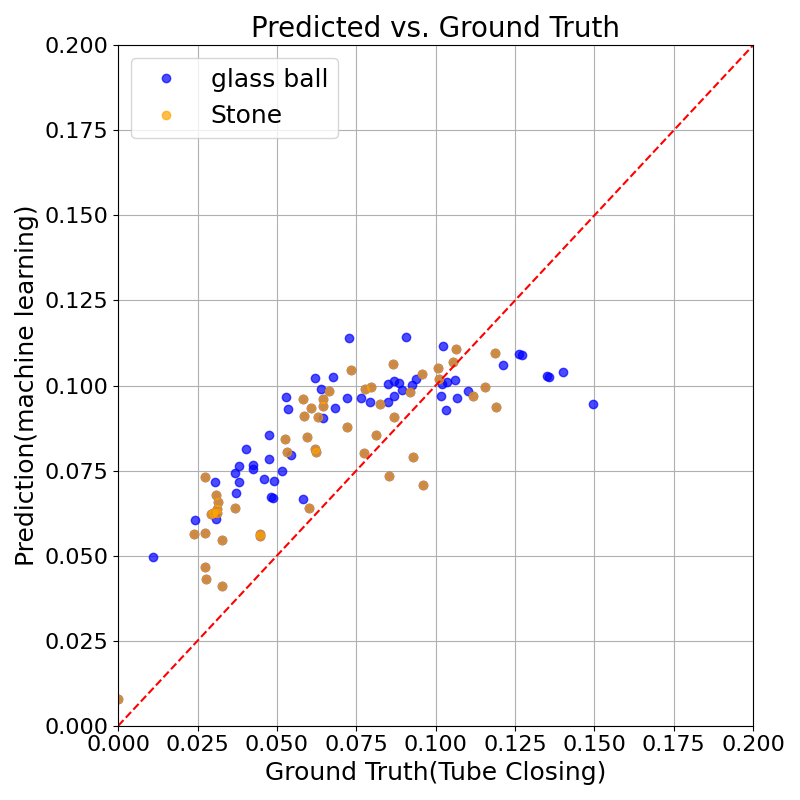
\includegraphics[width=0.4\linewidth]{pictures/results/predicted_vs_ground_truth_noerrorbars.png}
    \caption{縦軸が予測値を、横軸が実測値を示す。ゆえに、点群がy=xに近ければ近いほど精度が高いと判断される。}
    \label{fig:prediction_vs_ground_truth}
\end{figure}

\newpage
\subsection{課題}
これらテストデータに対する偏りとして、相体積率の最大値が0.15(正確には、2024年データにおいて0.149)というものがあげられる。ゆえに、0から0.15までの値をランダムに予測したり、適当な一次関数からのサンプルでもRMSEの率はそれほど高くはならない。このような議論を行う上では統計検定が必要である。平均すればある程度良い予測結果が得られる一方で、いくつかの欠点がある。まず一つに、機械学習の際、訓練データとテストデータ(実機)の評価が大きくずれる事象が数多く見られた。定性的に一定の類似性はみられるとはいえ、シミュレーションと実機ではデータにあまりに多くの差異がある可能性がある。\par
\begin{figure}[htbp]
    \centering
    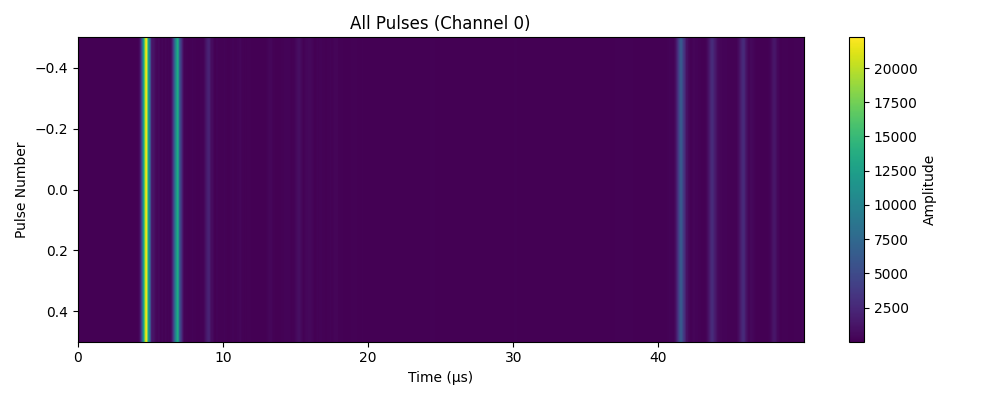
\includegraphics[width=0.5\linewidth]{pictures/explanation/solid_liquid7_processed_0img.png}
    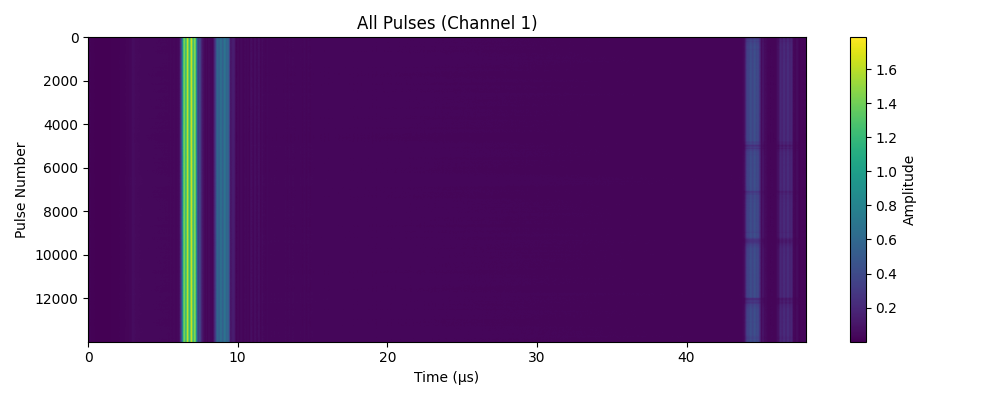
\includegraphics[width=0.5\linewidth]{pictures/explanation/P20240726-1600_processed_1img.png}
    \caption{シミュレーションと実機試験のデータの比較。両者ともに超音波画像法\ref{ultraimage}によって画像化してある。}
    \label{fig:noerrorbar}
\end{figure}
この二つの画像は、そのサンプルである。超音波パルスの幅や、多重反射が明瞭に確認できる回数などに違いが見て取れる。それでも一定の精度を得られたのは、情報処理のメカニズムにおいて、学習の過程でたまたま十分にロバストで実機データを処理するのにも使用可能な局所最適解・パターンを発見したからである可能性が高い。事実、学習率をさげて訓練を行った場合には、訓練データに対してよい精度を示しかつ安定的な学習を行った一方で実機データの値を適切に予測することができなくなった。
だが、それよりも重要なのは、予測に際し分散が非常に大きいということである。上記のグラフは平均値のみをプロットしたが、時間平均を計算する過程で評価できる分散の値も同時にプロットすると
\begin{figure}[htbp]
    \centering
    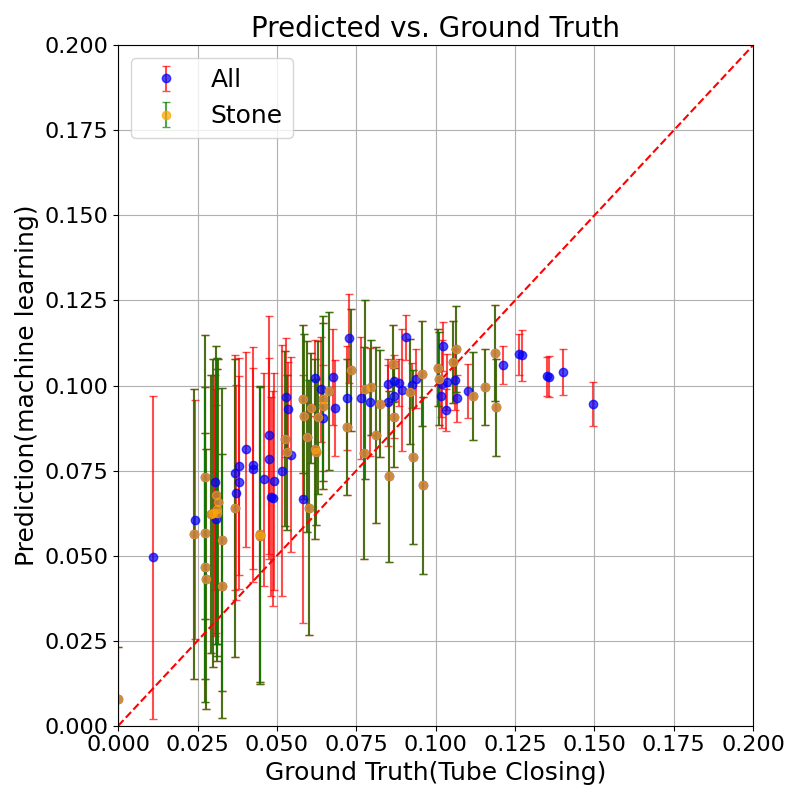
\includegraphics[width=0.5\linewidth]{pictures/explanation/predicted_vs_ground_truth_2.png}
    \caption{Caption}
    \label{fig:errorbars}
\end{figure}
のように、著しくError barが大きく表示されてしまうという問題点がある。これらへの考察として、トランスデューサの数が少ないからというものが挙げられる。機械学習とは統計的なパターン認識技術にすぎないので、予測とは尤もらしい予測とそれに付随する分散によって評価されるからであると考えられる。\par
一方で、実はこれら推定値はリアルタイムにおける相体積率を正しく推定しているという主張もある。実験では5秒間の測定を行っており、3 kHz回の測定の間に真の物理量は明らかに変動しうる。しかし、今回の場合算出したのは平均および分散、標準偏差である。
\subsection{問題解決の提案}
より信頼性の高いモデルを構築しようとした場合に重要なのは、ハイスピードカメラで計測した画像とシミュレーションの予測値を比較することだろう。
\chapter{結論}
\backmatter
\chapter{謝辞}
\bibliographystyle{junsrt}
\bibliography{reference}
\appendix\label{appendix}

\chapter{付録}
機械学習は統計的な手法であり、アルゴリズムの設計にもその性能評価にもいくつかの数学的準備を必要とする。ここでは、用いた議論や論拠の補足を行う。
\section{指標}
分類・回帰の性能評価に関する議論を行う。分類モデルに関しては精度・再現率・F値といった数々の指標が良く議論されている一方で、回帰タスクにおいては十分に行われていないようである。ここでは、その性能指標について、今回RMSEをMAEよりも好むかの理由について述べる。\par
そもそも、今回は固相体積率という連続値をとる量を推定する目的で研究が行われてきた。その理由は、構成方程式の精度を検証するためであった。誤差が生じる状況を大きく二分するとすれば、次の二つのケースが考えられる。
\begin{description}
    \item[1.] 全体的に中程度の誤差が出て、大きな誤差を取るものが極めて少ない
    \item[2.] 全体的に小程度の誤差が出て、一部のみ大きな誤差を取るものが存在する。
\end{description}
このうち、精度を検証する目的では全体的な中程度の誤差は、一部の大きな誤差よりも優先される。MAEではその誤差に対して線形な損失を割り当てるのに対し、MSEではその誤差の二乗の損失を割り当てる。それゆえ、L1Loss(MAE)よりもL2Loss(MSE)のほうが望ましい。さらに言えば、ある程度の誤差が許容されるのであればより高次のLossを用いるのさえ望ましい。MAEを利用しない理由はこれである。
\section{物性値}
物性値に関しては、現在に至るまでの数々の実験から再現可能な量が測定されてある。まず初めに、計算系において物性値を以下のように設定した。
\begin{table}[]
    \centering
    \begin{tabular}{c|c|c|c}
    \hline
         substance & Acoustic impedance & density & sound velocity \\
         \hline
         air&  0.00043 & 1.3 & 330\\
         water& 1.5 & 1000 & 1500\\
         glass & 18.9 & 2200 & 5300\\
         \hline
    \end{tabular}
    \caption{acoustic impedance used in the experiment}
    \label{tab:acoustic impedance}
\end{table}
\end{document}
